\section{Models of Memory}

Ebbinghaus is credited with a theory of memory and forgetting which has
withstood empirical study for over a century \cite{ebbinghaus}. It is known as
the power law of forgetting.  According to the power law of forgetting, the
strength of a memory after a time $t$ falls off exponentially: 

\begin{equation}
\label{eq:ebbinghaus}
 S(t) = ae^{-bt}
\end{equation}

In this model, $a$ is the initial strength of the memory, and $b^{-1}$ is a
decay rate.  The curve drawn by this function is known as the curve of
forgetting, which is depicted in Figure~\ref{fig:forgetting}.  If $a=1$, the
function may be interpreted as a probability function:

\begin{equation}
\label{eq:ebbinghaus}
 p(t) = e^{-bt}
\end{equation}

\begin{figure}[p!]
 \label{fig:forgetting}
 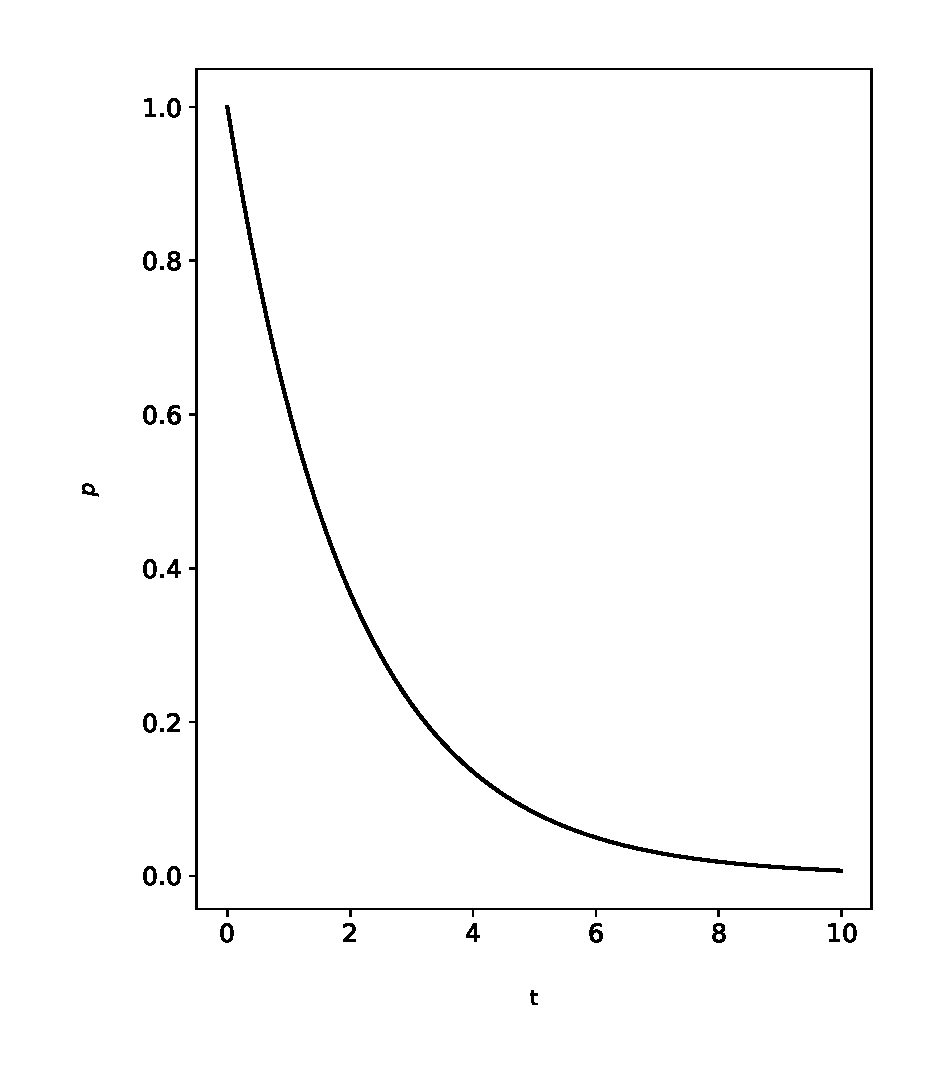
\includegraphics{fig/forgetting.eps} 
 \caption{The curve of forgetting}
\end{figure}

According to the theory, if the memory strength falls below a certain
threshold, then in the absence of any intervening information (that is,
information which re-activates the memory via association), the individual will
be unable to spontaneously recall the information.  In a probabilistic model,
one may set the threshold at .5 probability---the probability below which the
individual has more than likely forgotten the information. 

\section{ACT-R}

John Anderson developed a model for process-based learning which could provide
the foundation for an intelligent tutoring system \cite{anderson}.  He called
this Adaptive Control of Thought-Rational (ACT-R).  In ACT-R, there are goals,
akin to problem statements; and rules, or processes used to solve problems; and
finally facts, or knowledge utilized in the course of applying rules.  In this
regard, the structure of an ACT-R model resembles a logic program.  

In addition to this, however, Anderson added models for memory and forgetting
to support realistic recall probabilities and latencies.  The memory component
is based on Ebbinghaus' model of memory retrieval.  Anderson added a component
to explain memory re-activation of a memory.  According to Anderson's model, a
chunk of memory $i$ is re-activated (or additionally activated) to the extent
that other chunks of information (related concepts, words, ideas, etc.) which
have some association to $i$ are attended to.  This notion is captured in the
following equation:

\begin{equation}
\label{eq:anderson}
a_i = b_i + \displaystyle\sum_{i=j}^n w_j s_{ji}
\end{equation}

In this equation, known as the activation equation, the activation of a chunk
$i$ is equal to its base activation $b_i$, plus the products of the attentional
weights $w_j$ by the associative strength of $s_{ji}$ to other chunks.  This
provides an intuitive explanation for the manner in which recall of a target
chunk can be stimulated by dropping hints, using certain key words or phrases,
or mentioning related material. 

Practice has the effect of causing the base strength of the memory to increase,
and delays cause the strength of the memory to drop off:  

\begin{equation}
\label{eq:anderson}
b_i = \mathrm{ln} \Bigg( \displaystyle\sum_{j=1}^n t_j^{-d} \Bigg)
\end{equation}

Here, $t_j$ is the time since the jth practice of an item, and $d$ is a decay
rate. \ldots

Some concepts, particularly the notion of re-activation of memories, have been
borrowed from ACT-R and modified to fit the more coarse-grained intelligent
tutoring system presented in this work.  In particular, total problems rather
than individial processes will have probabilities of recall associated with
them.  Also, associative strenghts are established using a factor analysis.

\begin{figure}[p!]
 \label{fig:memory}
 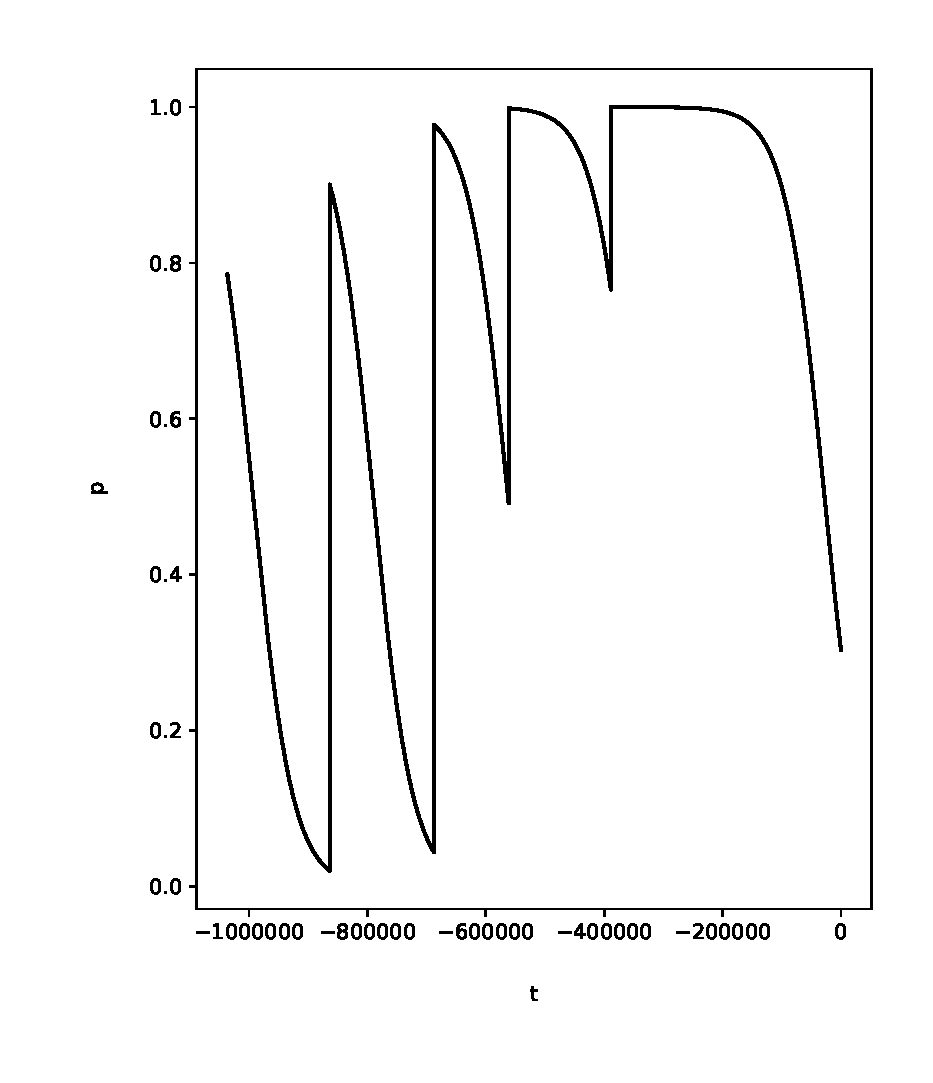
\includegraphics{fig/memory.eps} 
 \caption{Forgetting with re-activation}
\end{figure}

\section{Alterations to Memory Model}

A slight modification to this theory accounts for short-term memory and
short-term memorization, which allows for a small time window for the student
to enjoy a high probability of recollection before dropping off sharply, as in
the original curve:

\begin{equation}
\label{eq:modified}
 p(t) = \frac{1}{1 + e^{{m(t-\lambda)}}}
\end{equation}

In this equation, $\lambda$ is the lifespan of the memory; or, the amount of
time that passes until there remains only a .5 probability that the student
recalls the information.  The value $m$ is a parameter which controls the rate
of dropoff, much like the decay rate in Ebbinghaus' model.  An example curve
for this equation is given in Figure~\ref{fig:modified}.

\begin{figure}[p!]
 \label{fig:modified}
 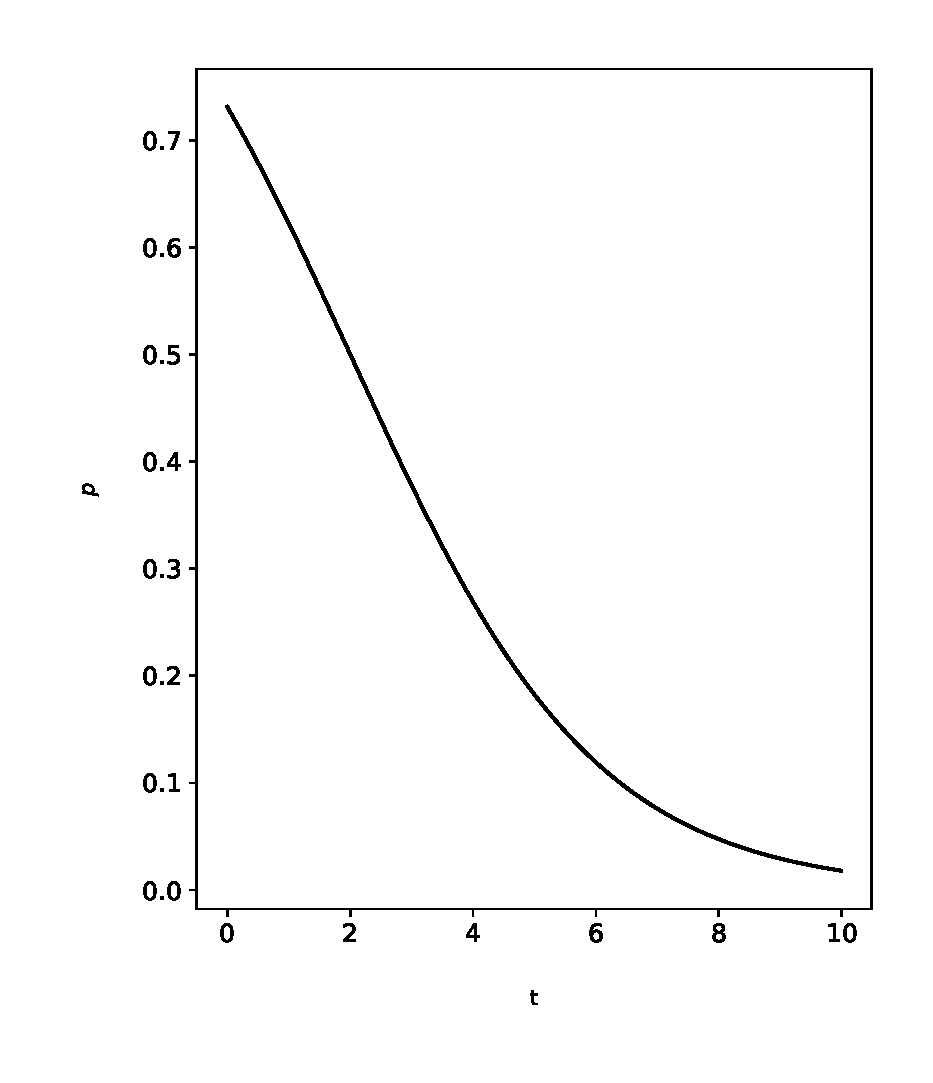
\includegraphics{fig/modified.eps} 
 \caption{The modified curve of forgetting}
\end{figure}

\section{Re-Activation}

To account for re-activation, a simple model for the extension of half-life
may be used: 

\begin{equation}
\label{eq:ebbinghaus}
 \lambda_n = \rho_s \lambda_{n-1}
\end{equation}

Here, $n$ refers to exposure or trial number $n$.  In the intelligent tutoring
system, this is the nth time that the student has seen the problem.
$\lambda_{n-1}$ is the former lifespan of the memory.  $\rho_s$ is a learning
rate, which is a parameter particular to the student; its domain is (1,
$\infty$].  The intuition captured by this formula is that with an increased
number of trials, the lifespan of the memory increases.

Apparently there is a difference in problems in the ease with which they are
learned.  An addendum to this can be used to account for individual differences
in problems: 

\begin{equation}
\label{eq:ebbinghaus}
 \lambda_n = \mu_i \rho_s \lambda_{n-1}
\end{equation}

Here, $\mu_i$ represents the memorability of the problem, or the ease with
which the problem solution can be committed to memory. 


% TODO: relationship to power law of learning or learning curve.
% TODO: show relationship between Anderson and this?

\subsection{Spacing Effect}

The spacing effect is the effect that the amount of time in between trials has
on the memorization of a chunk of memory.  In the above model, memorization is
interpreted as an increase in the lifespan of a memory.  If only a short amount
of time passes between the last trial, the effect will not be as great as if a
longer time has passed.  One consequence of this is that, according to the
spacing effect hypothesis, cramming is ineffective (where cramming is namely
repeating trials in short bursts).

The spacing effect can be accommodated in the memory model used by the
intelligent tutoring system.  We define a function for the dropoff:

\begin{equation}
  \label{eq:spacing}
  \sigma(t) = \rho_s(1 - e^{-t})
\end{equation}

\begin{equation}
\label{eq:ebbinghaus}
 \lambda_n = \sigma(t) \mu_i \rho_s \lambda_{n-1}
\end{equation}


